% -----
\chapter{Conclusion}

The work presented in this thesis is embodied in the Disciplined Disciple Compiler (DDC) which can be obtained from the \texttt{haskell.org} website. We have found it invaluable to develop the compiler alongside the source language and type system. Having a real compiler allows us to experiment with example programs that would be impractical to manipulate by hand, and we have been working on DDC since the very start of this project.

DDC is not yet `industrial strength', but it does have enough functionality to compile non-trivial programs. Screenshots from two of our test programs are below. The one on the left is a real-time, 2-dimensional particle collision simulation that uses a quad-tree to determine when two particles are close enough to possibly collide. The second is a simple ray tracer which uses a vector library based on our projection system. 

Developing these programs has given us insight into some of the strengths and weaknesses of our current system. In this chapter we briefly discuss our back-end implementation, identify opportunities for further work, summarise our contributions, and conclude.

\subsubsection{Gratuitous Screenshots}

\begin{tabular}{lll}
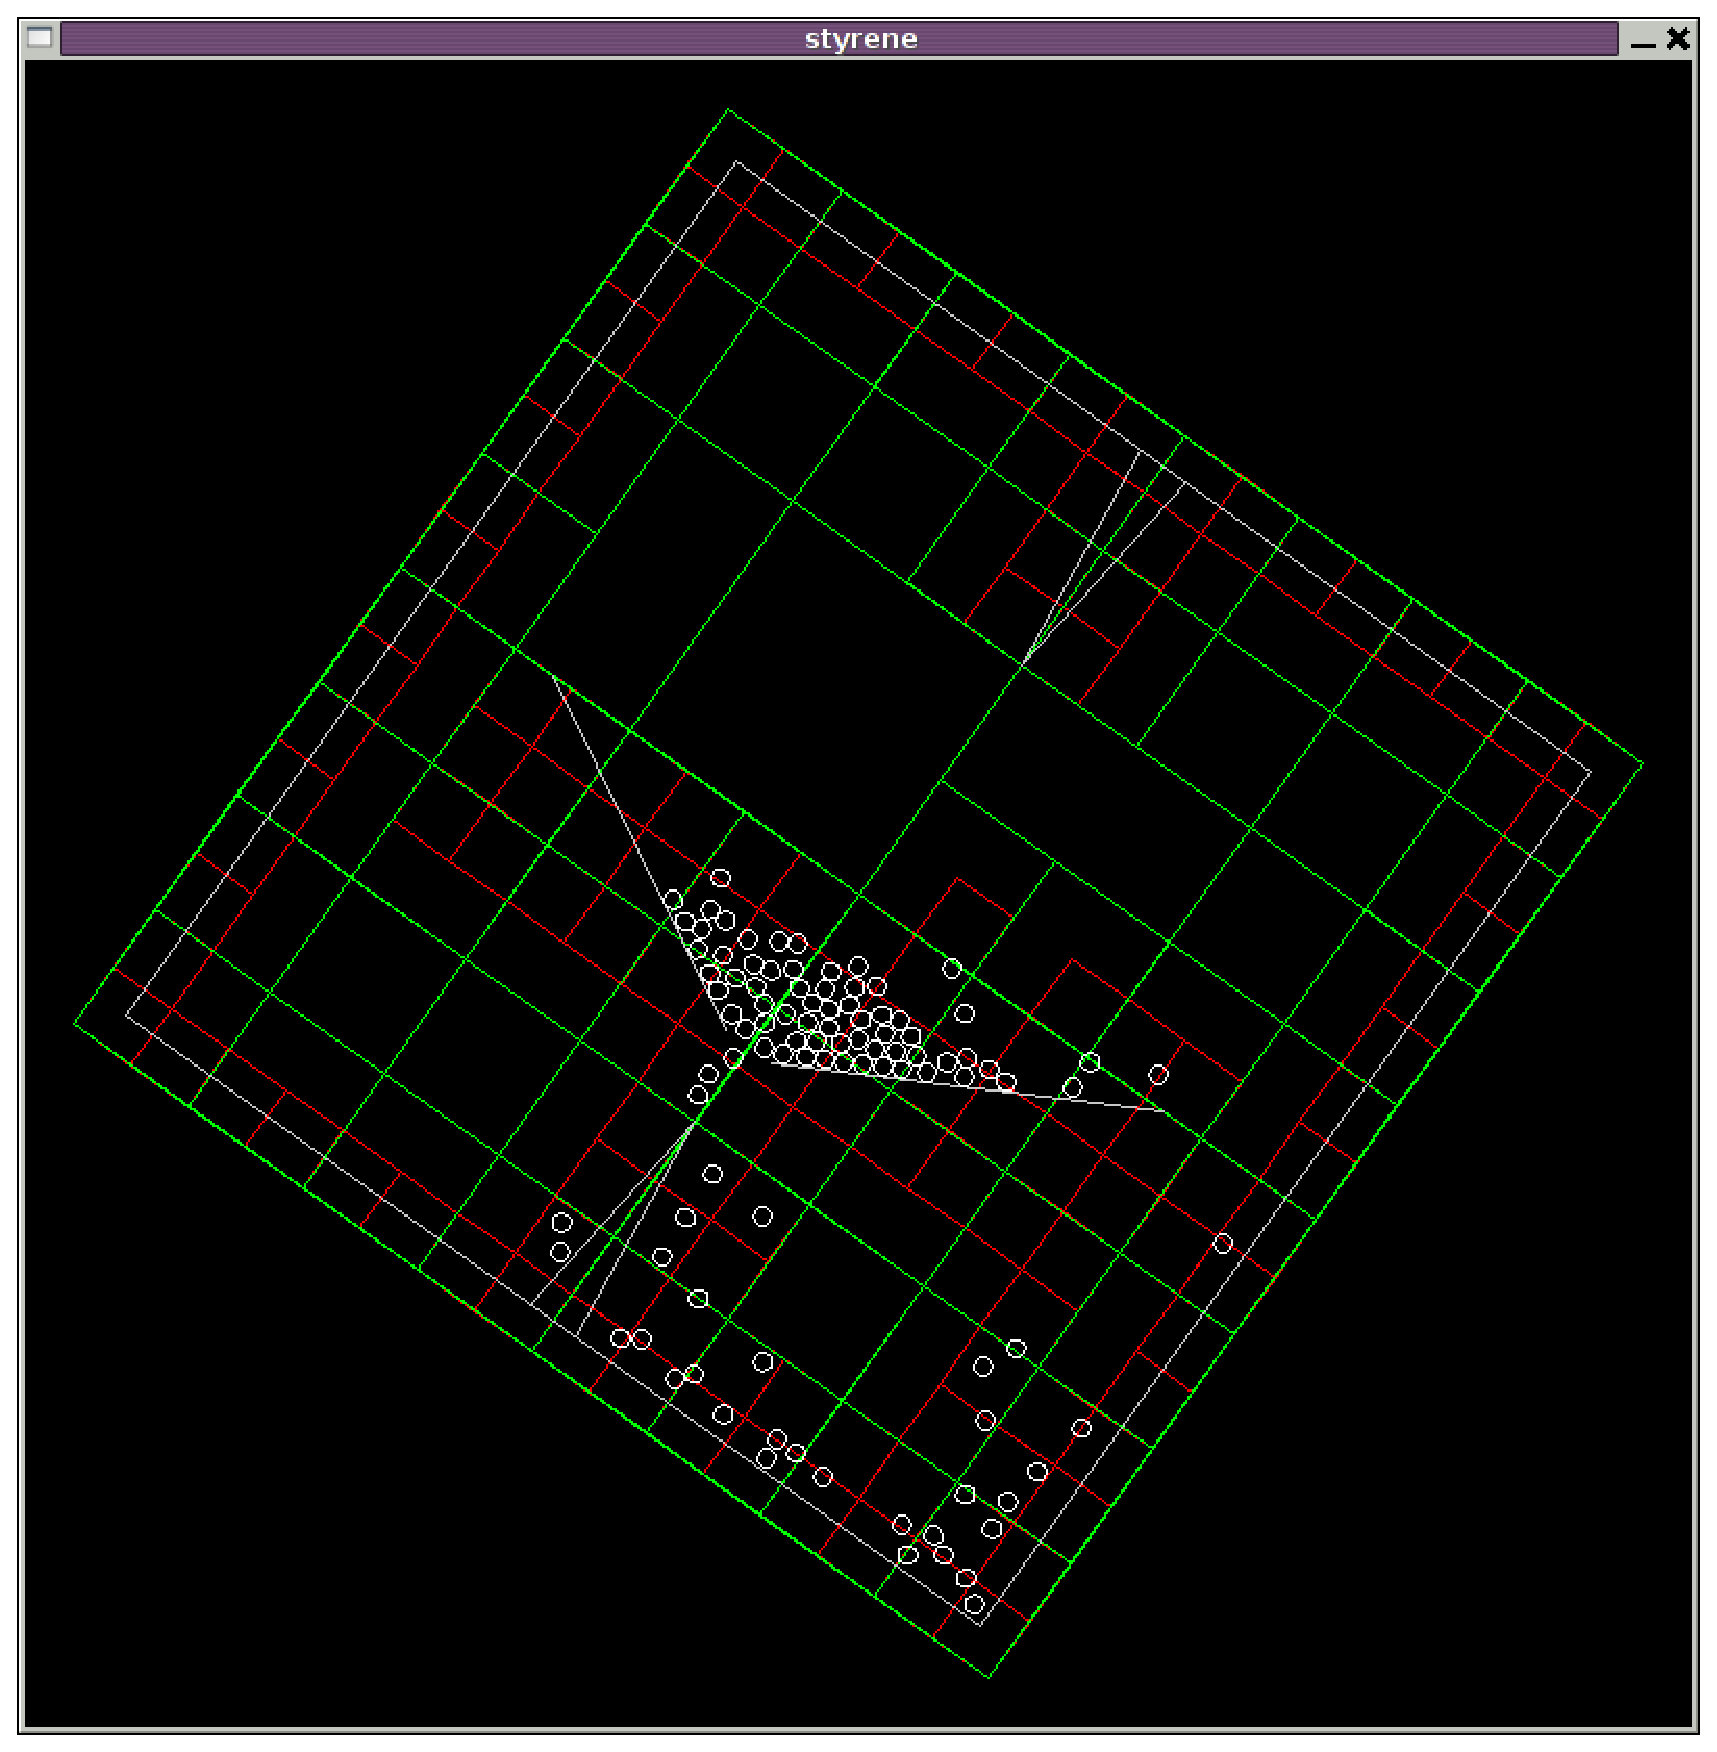
\includegraphics[scale=0.2]{5-Conclusion/Examples/fig/styrene}
&
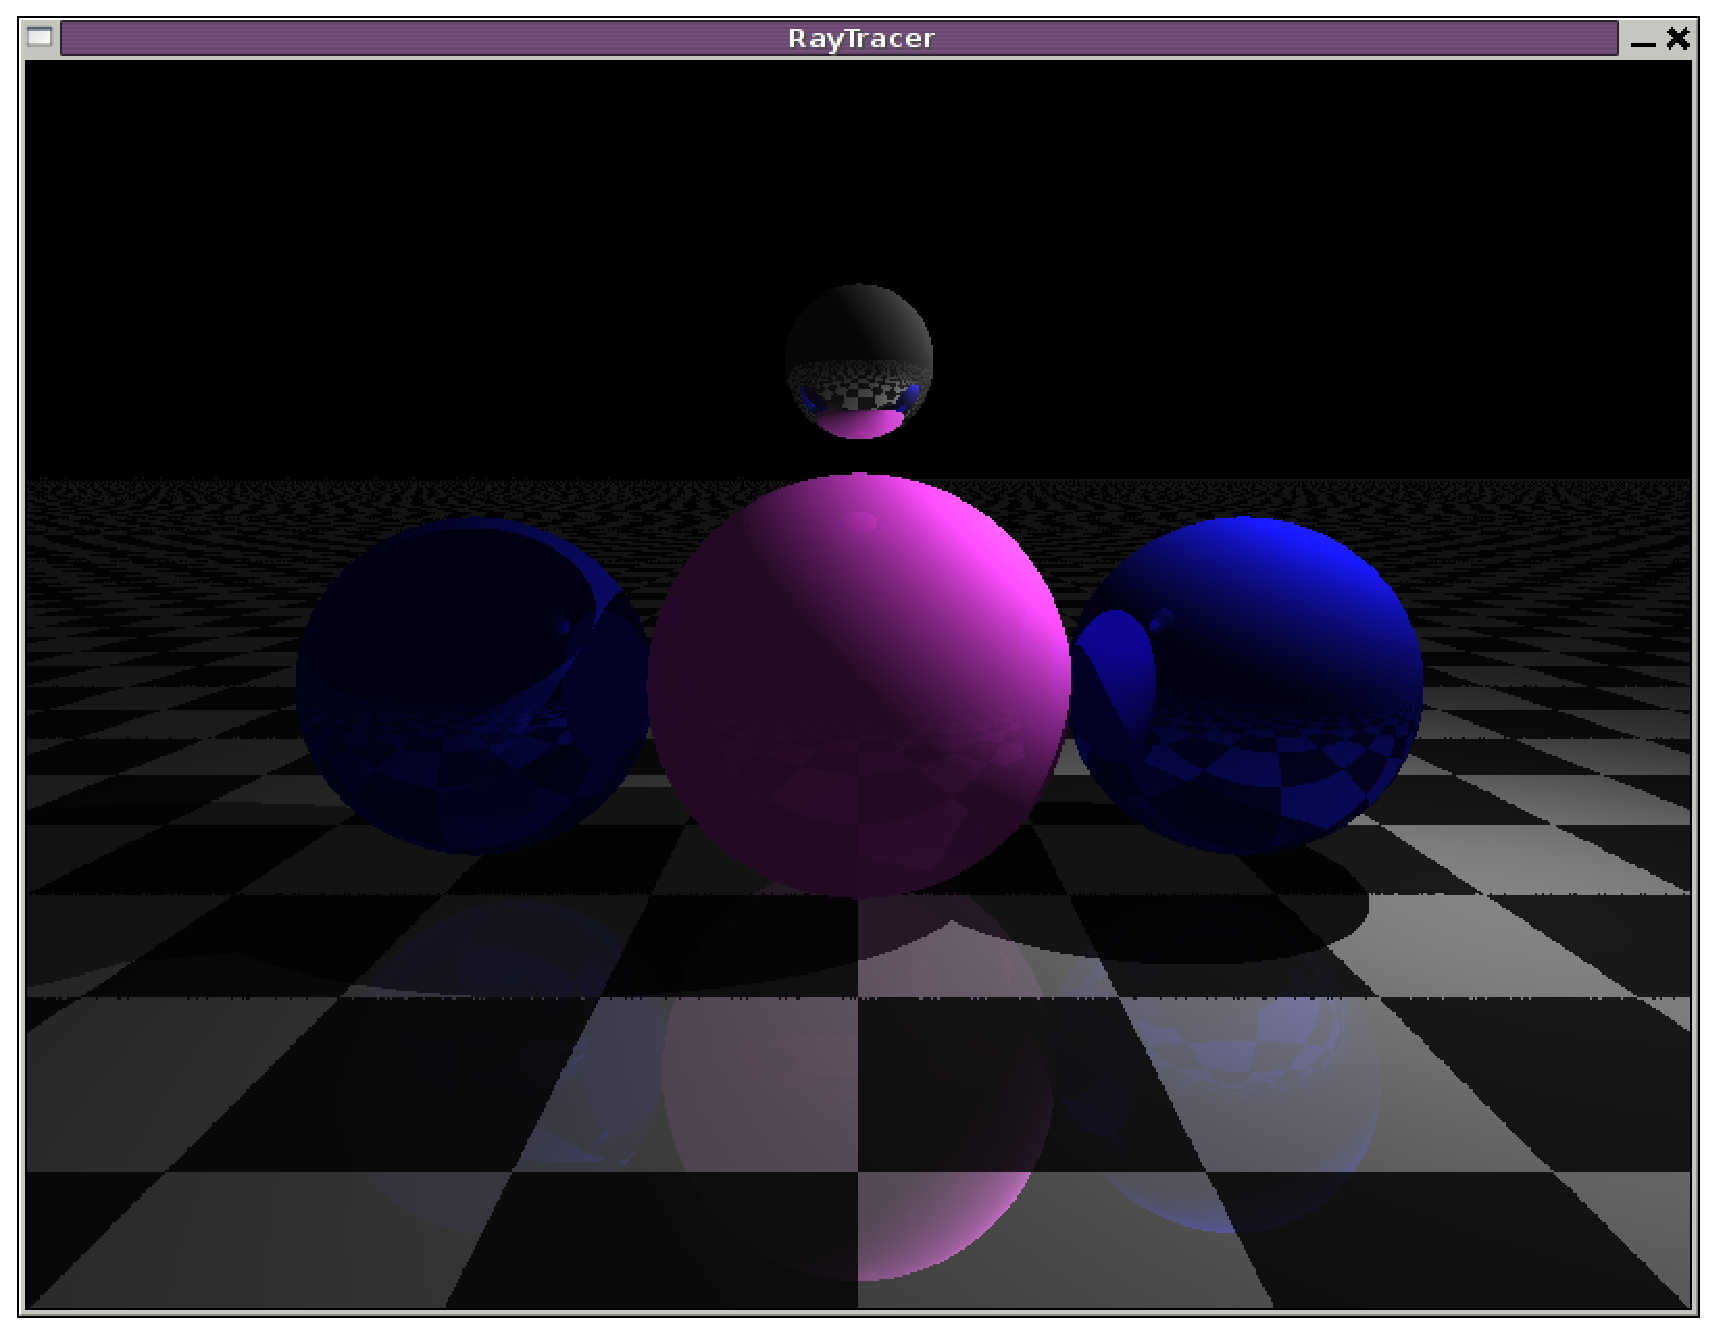
\includegraphics[scale=0.262]{5-Conclusion/Examples/fig/raytracer}
\end{tabular}




\clearpage{}
\section{Implementation}

DDC is written in Haskell with GHC extensions. It uses three intermediate representations: a desugared form of the source language; the core language presented in this thesis, and an abstract C-like language. We have used Parsec \cite{leigen:parsec} for the parser, and compile to ANSI C.

As the focus of our work has been on the type system and core language, we have not put a substantial amount of work into optimising the back end. However, we have gleaned a few points that may be of interest to others embarking on a similar endeavor. Although compiling via third party intermediate languages such as C$- -$ \cite{peyton-jones:portable-assembly-language} or LLVM \cite{lattner:llvm} is likely to produce better code in the long run, we feel that targeting C still has a place if the developer ``just wants to get something working''. The primary benefits are that a given developer will invariably know C already, and that implementions of primitive functions can be written directly. 

\subsection{Implementing thunks and laziness}

As Disciple uses call-by-value evaluation as default, we expect laziness to only be used occasionally. We desire straight-forward, C-like programs that do not make heavy use of higher order functions or partial application to run as fast as if they were actually written in C. For this reason we avoid the heavy encodings that are associated with compiling via an abstract machine, such as the STG machine 
\cite{peyton-jones:g-machine}.

After the core-level optimisations are finished, we perform lambda lifting to generate supercombinators \cite{hughes:thesis}. Each supercombinator is translated to a single C function. We handle partial application by building a thunk containing a pointer to the associated supercombinator, along with the provided arguments. This is the eval/apply method discussed in \cite{marlow:fast-curry}.

Thunks representing suspended computations are created with explicit calls to the $\isuspend$ function that was introduced in \S\ref{System:Effects:purification}. Thunks that represent numeric values are forced by the $\iforce$ function. Calls to $\iforce$ are introduced by the compiler during the local unboxing optimisation that was discussed in \S\ref{Core:Optimisation:floating-same-level}. We use \texttt{switch} statements to implement core-level case-expressions, and thunks that represent values of algebraic type are forced by extra alternatives that we add to these statements.

For example, the following expression:

\code{
	\mc{2}{$\kcase \ \ixx \ \kof$} \\
	& $\iNil$		& $\to \ ... \ \ialtOne \ ...$ \\
	& $\iCons \ x \ \ixs$	& $\to \ ... \ \ialtTwo \ ...$ \\
}

compiles to:

\begin{lstlisting}
  again:
  switch (_TAG(xx)) {
    case tag_Nil:   goto alt1;
    case tag_Cons:  goto alt2;
    case tag_INDIR: xx = ((Thunk*)xx)->next; goto again;
    case tag_SUSP:  xx = force(xx);          goto again;
    default:        ... error handling ...
  }
\end{lstlisting}

The tags \texttt{INDIR} and \texttt{SUSP} are common to all objects. When the tag of an object is inspected, if it turns out to be an indirection or suspension then it is followed or forced appropriately. The object is then reinspected by jumping back to the start of the \texttt{switch} statement. Note that we place the alternatives for indirections and suspensions last in the list. This ensures that the handling of lazy objects does not degrade the speed of programs that use mostly call-by-value evaluation. If the type of the object to be inspected is constrained to be direct, then we can omit the \texttt{INDIR} and \texttt{SUSP} alternatives and gain a slight speedup due to a smaller executable.

The primary advantages of this method are its simplicity and portability. The disadvantage is that we incur a function call overhead every time we force a thunk. This method is unlikely to ever match the efficiency a purpose built system based on the STG machine \cite{peyton-jones:g-machine}, but it works, and is significantly easier to implement.




\section{Limitations and possible improvements}

This section discusses some of the limitations that we have uncovered in our current system. Although we present ideas for addressing these limitations, they have not yet been fully developed or implemented. The limitations are presented in order, with the ones that we feel would most affect client programmers listed first. Most of these limitations were introduced earlier in this thesis, and we elaborate on them here as a guide for future work.


\subsection{Masking mutability constraints}
\label{Evaluation:Limitations:mutability-masking}

As mentioned in \S\ref{System:Effects:masking}, although we can mask effects on region variables that correspond to fresh objects, we cannot mask mutability constraints on the same variables. The classic example is a function that destructively updates a counter when calculating the length of a list, and then returns the counter. With effect masking, our current system gives this function the following type:

\code{
	$\ilength$
	& $::$		& $\forall a \ r_1 \ r_2. \ \iList \ r_1 \ a \lfuna{e_1} \iInt \ r_2$ \\
	& $\rhd$	& $\iRead \ r_1$ \\
	& $,$		& $\iMutable \ r_2$
}

For this example we can work around the problem by copying the counter value before returning it. This invokes the $\iShape$ constraint discussed in \S\ref{System:TypeClassing:copy-and-update}, and allows the resulting value to have a differing mutability. We expect to solve the general problem by introducing closure information into the core language, and then using a similar mutability masking mechanism to the one outlined by Gupta in \cite{gupta:functional-encapsulation}.

\clearpage{}
\subsection{Blocked regions and region sums}
\label{Evaluation:Limitations:blocked-regions}

The following program is rejected by our system:

\code{
	\mc{3}{$x = 5$}	
	\\[1ex]
	\mc{3}{$\ifun \ ()$} \\
	\quad $= \kdo$	& $y = 23$	\\
			& ... \\
			& $y := 42$ \\
			& $\kif \ ... \ \kthen \ x \ \kelse \ y$
}

As $x$ is defined at top level it defaults to being constant, and as $y$ is updated it must be mutable. However, both $x$ and $y$ are returned by the if-expression, so our system requires them to have the same type. This creates a mutability conflict, so the program is rejected.

Our work-around is to explicitly copy either $x$, $y$, or both. This solves the immediate problem, but is clumsy and could result in a considerable run-time overhead when dealing with larger structures.

Note that if we could guarantee that the result of the if-expression was treated as \emph{neither} constant nor mutable, then we could allow the above program. As discussed in \S\ref{System:Effects:liftedness}, we view mutability as the capability of an object to be updated, and constancy as the capability of suspending a computation that reads it.  We have in mind to introduce a new constraint, $\iBlocked$, which prevents a region variable from being additionally constrained as either $\iConst$ or $\iMutable$.

However, we do not want the $\iBlocked$ constraint to `leak' into the type of $x$. The fact that we choose between $x$ and a mutable value does not mean there is any danger of suspending a function that reads $x$ directly. Say $x$ and $y$ have the following types:

\code{
	$x$	& $:: \iInt \ r_1 \rhd \iConst \ r_1$ \\
	$y$	& $:: \iInt \ r_2 \rhd \iMutable \ r_2$
}

We would prefer to leave $r_1$ and $r_2$ as constant and mutable respectively, and use a \emph{region sum} to express the fact that the result of $\ifun$ could be in either region $r_1$ or $r_2$. The full type of $\ifun$ would then be something like:

\code{
	$\ifun$	& $::$		& \mc{2}{$\forall \ c_1 \ r_2 \ r_3. \ () \lfuna{c_1} \iInt \ r_3$} \\
		& $\rhd$	& $c_1$ & $\tme x : \iInt \ r_1$ \\
		& \ ,		& $r_3$ & $\tme r_1 \lor r_2$ \\
		& \ ,		& \mc{2}{$\iConst \ r_1$} \\
		& \ ,		& \mc{2}{$\iBlocked \ r_3$} \\
}

The constraint $r_3 \tme r_1 \lor r_2$ is read: ``$r_3$ might include objects from $r_1$ or $r_2$'', with the ``or'' being non-exclusive. The literature on union typing, such as \cite{dunfield:intersections-and-unions}, may provide clues on how to implement this.

\subsection{Bounded quantification and effect strengthening}

In section \S\ref{Core:Extensions:Bounded} we discussed bounded quantification and how it is included in our core language. We added this feature so that we can directly express the types inferred by our Talpin-Jouvelot style inference algorithm. However, we are not convinced that bounded quantification (beyond type class constraints) is intrinsically necessary. We feel this way because there is never an operational need for the effect of one parameter function to be larger than another.

As discussed in \S\ref{System:Effects:constraint-strengthening}, effect variables serve to propagate the effect of a parameter into to the manifest effect of the overall function. This mechanism is used to express the fact that a higher order function may invoke its parameter, and our optimising transforms must be aware of this. The only time we need to constrain the effect of a parameter function is when we suspend an application of it, and we do this with purity constraints via the type classing system.

The fact that a function such as $\ifoo$ from \S\ref{System:Effects:constraint-strengthening} has a $\tme$ constraint on its parameter effect is an artefact of the bidirectional nature of Hindley-Milner type inference. This is related to the poisoning problem which is mentioned in \cite{benton:monads-effects-transformations} and discussed in \cite{wansbrough:once-upon-a-polymorphic-type}. Both \cite{wansbrough:once-upon-a-polymorphic-type} and \cite{benton:monads-effects-transformations} report that subtyping can be used to remedy this problem, but \cite{wansbrough:once-upon-a-polymorphic-type} concerns usage analysis and not effects, and \cite{benton:monads-effects-transformations} does not consider effect polymorphism. In \cite{benton:relational-semantics-effect-transformations} Benton \emph{et al} extend the system presented in \cite{benton:monads-effects-transformations} with region variables, but do not discuss type inference.

More work is needed to determine whether the effect (and closure) constraints on the types of higher order functions can always be strengthened. The goal would be to either eliminate the need for bounded quantification in the core language, or to determine why this can not, or should not, be done.


\subsection{Polymorphism, data sharing, and constraint masking}
\label{Evaluation:Limits:sharing-and-constraint-masking}

Suppose we wish to define a type class to help compute the areas of geometric figures. The obvious definition would be:

\code{
	\mc{4}{$\kclass \ \iArea \ a \ \kwhere$} \\
	& $\iarea$	& $::$		& $\forall r_1. \ a \lfuna{e_1} \iFloat \ r_1$ \\
	&		& $\rhd$	& $e_1 = \iReadT \ a$
}

This definition says that an instance of the $\iarea$ function produces a float into the fresh region named $r_1$, and is permitted to read its argument. Here is a data type to represent our figures:

\code{
	\mc{3}{$\kdata \ \iFigure \ r_1$} \\
	& $=$	& $\iRectangle \ (\iFloat \ r_1) \ (\iFloat \ r_1)$ \\
	& $|$	& $\iCircle \ (\iFloat \ r_1)$ 
}

The parameters of $\iRectangle$ are its width and height, and the parameter of $\iCircle$ is its radius. The area of a rectangle is its width multiplied by its height, and the area of a circle is $\pi$ times its radius squared:

\code{
	\mc{5}{$\kinstance \ \iArea \ (\iFigure \ r_1) \ \kwhere$} \\
	& \mc{5}{$\iarea \ \ifig$} \\
	& \mc{5}{$\ = \kcase \ \ifig \ \kof$} \\
	& & & $\iRectangle \ w \ h$	& $\to w \ * \ h$ \\
	& & & $\iCircle \ r$		& $\to \ipi \ * \ r^2$
}

Unfortunately, this is not a valid instance of $\iArea$. The trouble is that the constant $\ipi$ is free in the closure of $\iarea$, but this information is not present in the class definition. If we assume $\ipi$ is defined at top level and has the type $\iFloat \ r_5$, then our instance function has type:

\code{
	$\iarea_{\iFigure}$	
	& $::$		& $\forall r_1 \ r_2. \iFigure \ r_1 \lfuna{e_1 \ c_1} \iFloat \ r_2$ \\
	& $\rhd$	& $e_1 = \iRead \ r_1$ \\
	& $,$		& $c_1 = \ipi : \iFloat \ r_5$
}	

Although we \emph{could} go back and widen the class definition so that all instances of $\iarea$ are assumed to refer to $\ipi$, this is an unsatisfying solution. How could we decide \emph{a priori} which constants would be needed? For example, the surface area of a torus is $4 \pi^2Rr$, where $r$ and $R$ are the inner and outer radii. When determining such an area we would prefer to use a constant $\ipiTwo$ instead of computing the value of $\pi^2$ each time. Should we include just $\ipi$ and $\ipiTwo$ in the class definition, or will we need other constants as well?

In essence, our current system exposes too much useful information about the sharing properties of data. Although we need this information to reason about mutability and to perform effect masking, we sometimes want to ignore it in the interests of polymorphism. Using the language of \cite{neergaard:nonlinearity-and-amnesia}, it is nonlinearity and `amnesia' which make a type system work. A given system must be able to forget about the exact details of the program, otherwise testing for well-typedness degenerates to simply running the program and checking for failure.

A seemingly obvious solution is to erase closure terms that refer to constant regions, but we have to carefully consider possible interactions with other extensions to the language. For example, if we allow masking of $\iMutable$ constraints as per \S\ref{Evaluation:Limitations:mutability-masking}, then what about masking of $\iConst$ constraints as well? For example, say we have a function of the following type:

\code{
	$\ifun$	& ::		& $() \lfuna{c_1} \iFloat \ r_1$ \\
		& $\rhd$ 	& $c_1 = x : \iFloat \ r_1$ \\
		& ,		& $\iConst \ r_1$ 
}

As $r_1$ is constant, we could argue that the constraint on $c_1$ should be erased. Assuming that $x$ is not in the type environment, this would also allow $r_1$ to be generalised:

\code{
	$\ifun$	& ::		& $\forall r_1. \ () \to \iFloat \ r_1$ \\
		& ,		& $\iConst \ r_1$ 
}

Now, this type doesn't look too different from the type of $\ilength$ in \S\ref{Evaluation:Limitations:mutability-masking}. If we followed the reasoning presented there then we might like to (erroneously) mask the constancy constraint as well:

\code{
	$\ifun_{\ibad}$	
		& ::		& $\forall r_1. \ () \to \iFloat \ r_1$ 
}

However, this in invalid. With this type there is nothing stopping us from updating the return value. The point is that a constancy constraint does not \emph{just} mean that a given object should not be updated, it means that it should not be updated because other expressions may refer to it in ways that are not visible in our type information.

This brings us back to our discussion of region allocation from \S\ref{Core:Language:lazy-evaluation}. Recall that we do not currently use regions for allocation, or more importantly \emph{deallocation}. This is because a `value' of type $\iInt \ r_1$ may be represented by a thunk, and that thunk may hold references to objects in regions which are not present in its type. We cannot currently perform region allocation because our type system does not provide us with information about what objects might be invisibly referenced by thunks. Knowing that those objects are \emph{constant} is not enough, what we actually need is a list of region variables that have escaped our analysis and must be assumed to be shared at top-level. Importantly, this is also the same property we need to consider in our type class example.

We have in mind to introduce a new region constraint $\iShared$ that expresses this property. We would also introduce a constraint $\iSharedT$ that refers to all the region variables in a particular value type, and another $\iSharedC$ that refers to region variables in a closure.

Our $\isuspend$ function would then have type:

\code{
	$\isuspend$
	& $::$		& $\forall a \ b. \ (a \lfuna{e_1 \ c_1} b) \to a \to b$ \\
	& $\rhd$	& $\iPure \ e_1$ \\
	& ,		& $\iSharedT \ a$ \\
	& ,		& $\iSharedC \ c_1$ 
}

This type expresses the fact that the closure of the parameter function, along with the value of type $a$, is still reachable after this function returns. Neither $c_1$ or $a$ are present in the type $b$, but the core language could use the sharing constraints on them to ensure that they are not region-allocated.

\subsection{Witnesses of no aliasing}
\label{Evaluation:Limits:aliasing}

As discussed in \S\ref{Core:Optimisation:effects-and-region-aliasing}, if the core translation of a function has two region parameters $r_1$ and $r_2$ then we must assume that objects in the corresponding regions may alias. This prevents us from reordering bindings with effects such as $\iWrite \ r_1$ and $\iRead \ r_2$. A natural extension would be to add a new witness constructor $\iMkNoAlias$, and use a witness of kind $\iNoAlias \ r_1 \ r_2$ to express the fact that objects in regions named $r_1$ and $r_2$ are guaranteed not to alias. The optimiser could then use such witnesses to prove that effects on these regions do not interfere.

If two region variables are introduced at the same point, the generation of a $\iNoAlias$ witness for them is straightforward. We could extend the letregion expression so that multiple region variables can be introduced, and require that witnesses of no aliasing are created at the same point. For example:
\begin{tabbing}
	MMMM \= MMMMM \= x \= MMMM\kill
	\> $\kletregion$	\> $\{ \ r_1, r_2 \ \}$ \\
	\> $\kwith$ 
		\> $\{$ \> $w_1 = \iMkMutable \ r_1$ \\ 
	\>	\> 	\> $w_2 = \iMkMutable \ r_2$ \\
	\>	\>	\> $w_3 = \iMkNoAlias \ r_1 \ r_2 \}$  \\
	\> $\kin$ ...
\end{tabbing}

However, if the $\iNoAlias$ constructor only has two region parameters, then the number of witness we might want to create is quadratic in the number of region variables introduced by the letregion expression. It may be better to extend the syntax of kinds so they can contain sets of region variables. This would complicate the type system, but it is an orthogonal extension. We could also use this functionality to reduce the multitude of other sorts of witnesses.  For example, by using a single witness of kind $\iMutable \ \{ r_1, r_2, r_3 \}$ instead of three separate ones.


\subsection{Should we treat top-level effects as interfering?}
\label{Evaluation:Limits:top-level-effects}

From a utopian viewpoint, effects such as $\iFileSystem$, $\iConsole$ and $\iNetwork$ should not interfere, but in practice they do. On a unix based system, data written to the special file \texttt{/dev/stdout} appears on the console, so in general we should not reorder calls to library functions such as $\iwriteFile$ and $\iputStr$.\footnote{With the meanings of these functions being the same as in Haskell.}

However, as we allow programmers to define their own effect constructors, we can forsee use-cases for embedded systems that incorporate effects such as $\iMotionSensor$, $\iRobotArm$, $\iBlinkyLight$ etc. Although $\iMotionSensor$ and $\iRobotArm$ would likely interfere, perhaps $\iMotionSensor$ and $\iBlinkyLight$ would not.

It would be straight-forward to allow the programmer to define their own effect interference relationships. This seems like a ``fun'' extension, but we are not sure how useful it would be in practice. For now, we treat all top level effects as interfering.


\subsection{Add witnesses to write effects}

In the type system for our core language, there is nothing that directly links the fact that write effects must only act on mutable regions. We rely on the signatures of primitive functions such as $\iupdateInt$ to contain both the mutability constraint and the write effect, but do not enforce it. We could perhaps change the kind of the $\iWrite$ constructor to require a witness that the region written to is mutable, that is:

\code{
	$\iWrite :: \Pi (r_1 : \%). \iMutable \ r_1 \to \ !$
}

We have not yet thought of a use-case where a programmer would desire a region to be mutable in the absence of a write effect, or import a primitive function that performs a write but does not require mutability. However, we have avoided giving $\iWrite$ the above kind because it would noticeably increase the volume of type information in the core program. An alternative would be to emit a compiler warning if a primitive function was defined with one but not the other, but this is more of an \emph{ad-hoc} solution. 


\subsection{A better type for $\iforce$}
\label{Evaluation:Limits:force}
In \S\ref{Core:Optimisation:floating-same-level} we avoided assigning a type to $\iforce$ because the only sensible type we can give it is $\forall a. \ a \to a$, and that's not particularly useful. We wish to encode the fact that the resulting value is guaranteed not to be represented by a thunk, but we do not have a way of doing so. For example, if we limited $\iforce$ to act on integers then we might try:

\code{
	$\iforce$	
	& $::$		& $\forall r_1. \ \iInt \ r_1 \to \iInt \ r_1$ \\
	& $\rhd$	& $\iDirect \ r_1$	
}

However, this does not work because we are expecting to apply $\iforce$ to objects that are constrained to be in $\iLazy$ regions. 

\clearpage{}
Using a different region variable in the parameter and resulting type does not work either:

\code{
	$\iforce$	
	& $::$		& $\forall r_1 \ r_2. \ \iInt \ r_1 \to \iInt \ r_2$ \\
	& $\rhd$	& $\iDirect \ r_2$	
}

With this type, the link between the input and output region variables is lost. If we apply $\iforce$ to an integer that is constrained to be mutable, then this constraint will not be present on the resulting type. It appears as though we need a way to relate the region variables $r_1$ and $r_2$ in a way that maintains all possible region constraints except $\iLazy$. In some senses, this is similar to the problem that the $\iShape$ constraint solves, which is discussed in \S\ref{System:TypeClassing:copy-and-update}. We could perhaps write something like:

\code{
	$\iforce$	
	& $::$		& $\forall r_1 \ r_2. \ \iInt \ r_1 \to \iInt \ r_2$ \\
	& $\rhd$	& $\iLazyToDirect \ r_1 \ r_2$ \\
	& ,		& $\iLazy \ r_1$ \\
	& ,		& $\iDirect \ r_2$ \\
	& ,		& $\iAlias \ r_1 \ r_2$ \\
	
}

The type inferencer would use the $\iLazyToDirect$ constraint to ensure that all constraints placed on $r_1$ other than $\iLazy$ were propagated to $r_2$, and all constraints placed on $r_2$ other than $\iDirect$ were propagated to $r_1$. We would need the extra constraint $\iAlias \ r_1 \ r_2$ in the event our system also contained the $\iNoAlias$ witnesses discussed in \S\ref{Evaluation:Limits:aliasing}.

The question is then how to reflect this $\iLazyToDirect$ constraint in the core language. We could perhaps use a higher kinded witness constructor to convert witnesses on $r_1$ to witnesses on $r_2$. Something like:

\code{
	\mc{3}{$\iMkLazyToDirectConv$} \\
	& $::$	& $\forall (k : \% \to \Diamond, \ k \ne \iLazy).$ \\
	&	& $\Pi r_1 \ r_2. \ \iLazyToDirect \ r_1 \ r_2 \to k \ r_1 \to k \ r_2$
}

This encodes the fact that if an object in a region named $r_1$ is forced, and then considered to be in a fresh region named $r_2$, then any property of the initial object is also a property of the resulting one, except for the possibility of being a thunk. However, as we do not have any experience with the associated type inference or core-level transforms we cannot comment on its practicality.


\section{Summary of Contributions}

\begin{itemize}
\item	I present a system that integrates region, effect and closure typing into a unified whole and uses type classes to express mutability and purity constraints. To my knowledge, the system in this thesis is the first to apply mutability constraints to region variables, or purity constraints to effect terms.

\item	I describe how laziness and arbitrary destructive update can be used sanely in the same program. This is done by applying purity constraints to the visible effects of suspended function applications, and satisfying these constraints by requiring objects read by the function to be constant. This ensures that impure function applications are not suspended, as the behavior of a program which did so would likely be incomprehensible to both the programmer and compiler.

\item	I present a System-Fc style core language that includes region, effect and closure information. I show how to encode information about mutability and purity using dependently kinded witnesses. 

\item	I describe the behaviour of a Talpin-Jouvelot style effect typing system when applied to higher order functions. I show how some $\tme$ constraints can be strengthened to equalities, but others cannot. Strengthening effect constraints allows the volume of type information in the core program to be reduced.

\item	I show how $\iShape$ constraints can be used to define type classes such as $\iEq$ and $\iCopy$. These constraints are used to require the parameter and return types of a function to have the same overall value type, while allowing the contained region and mutability information to vary.

\item	I discuss how $\iLazy$ and $\iDirect$ constraints can be used to track which objects might be represented as thunks. I show how to use this information to optimise programs that use mostly call-by-value evaluation.

\item	I discuss the concept of material region variables and show how this concept can be used to trim the majority of information out of closure terms. 

\item	I present pull-back projections and show how they can be used to eliminate the need for ML style mutable references. Using pull-back projections is preferable because ML style references pollute the value types of functions and data structures that use them, which can lead to a large amount of refactoring when developing programs.

\item	I describe how to perform Hindley-Milner style type inference without prior knowledge of the binding dependency graph. If the program uses type directed projections then this graph is not obtainable \emph{a priori}, because the instance function to use for each projection depends on the type of the value being projected.

\end{itemize}

\section{The Hair Shirt}

When I started this project back in 2004, one of the first things I came across were the slides for Simon Peyton Jones's 15 year Haskell retrospective entitled ``Wearing the Hair Shirt'' \cite{peyton-jones:wearing-the-hair-shirt}. When I looked up what a ``hair shirt'' was, it turned out to be a device of penance. Certain practitioners of the Christian faith wear (or wore) shirts made out of animal hair, because they are uncomfortable, and help to isolate the wearer from worldly passions.

Designing programming languages is almost too much fun. In the words of Aleister Crowley: ``We ignore what created us; we adore what we create''. It is all too easy to come up with a reasonable idea, fall in love with it, then begin to treat that idea as the one true way of solving any particular problem. Slide 41 of Wearing the Hair Shirt is titled ``What really matters?''. Four things are listed: Laziness, Purity and Monads, Type Classes, and Sexy Types. ``Laziness'' has a big red cross through it, and ``Purity and Monads'' are listed as one thing. I thought about that for some time, and that thinking turned into this thesis.

Five years later, I'd argue that in the context of functional programming, laziness and monads are merely tools, not universal truths. Purity is important to the extent that it reflects an understanding and control over side effects, and type classes and Sexy Types are one and the same. What matters, at least the way I see it, is the Curry-Howard isomorphism, but everyone knew that already.

I find the fact that we can leverage the Curry-Howard isomorphism to express relationships between region, effect and closure information to be highly reassuring. The core axioms, such as the fact that a read of a constant region is pure, are expressed in the kinds of witness constructors. The ambient type system does the rest.

The concrete implementation of DDC still has some wrinkles, but all the ones I know about are cosmetic and do not represent flaws in the overall approach or theory. The type system in this thesis, with its regions, effects, closures and various constraints is large in volume, but the various parts share much common ground. The type inferencer took a long time to work out, mainly because when I started I didn't know what I was doing, but the end result is surprisingly straightforward. 

If I were to distill this thesis into one single point, it would be that the distinction between ``pure'' and ``impure'' languages is an artificial one. As we can express information about effects and mutability directly in the type system, using a standard framework, the difference between pure and impure is no greater than the difference between $\iBool$ and $\iFloat$. Effect typing, closure typing, type classing, regions, dependent kinds and projections were all invented by other, eminently clever people. I've spent the last while pasting them together into a pleasing collage and smoothing out the corners. Now the world seems shiny and new.





\clearpage{}

\rule{0em}{10em}

\begin{center}
                                  14

          {Kappa-Epsilon-Phi-Alpha-Lambda-Eta Iota-Delta}

                            ONION-PEELINGS\footnote{An excerpt from The Book Of Lies, Aliester Crowley, 1913.}
\end{center}

\begin{tabbing}
MMMMMM \= M \= MMMMMMMMMMMMMMMMMMMMMMMMMM \kill
\>  The Universe is the Practical Joke of the General \\
\>  \> at the Expense of the Particular, quoth FRATER \\
\>  \> PERDURABO, and laughed. \\
\>  But those disciples nearest to him wept, seeing the \\
\>  \> Universal Sorrow. \\
\>  Those next to them laughed, seeing the Universal \\
\>  \> Joke. \\
\>  Below these certain disciples wept. \\
\>  Then certain laughed. \\
\>  Others next wept. \\
\>  Others next laughed. \\
\>  Next others wept. \\
\>  Next others laughed. \\
\>  Last came those that wept because they could not \\
\>  \> see the Joke, and those that laughed lest they \\
\>  \> should be thought not to see the Joke, and thought \\
\>  \> it safe to act like FRATER PERDURABO. \\
\>  But though FRATER PERDURABO laughed \\
\>  \> openly, He also at the same time wept secretly; \\
\>  \> and in Himself He neither laughed nor wept. \\
\>  Nor did He mean what He said. \\
\end{tabbing}




